% Options for packages loaded elsewhere
\PassOptionsToPackage{unicode}{hyperref}
\PassOptionsToPackage{hyphens}{url}
\PassOptionsToPackage{dvipsnames,svgnames,x11names}{xcolor}
%
\documentclass[
  10pt,
  dvipsnames,enabledeprecatedfontcommands]{scrartcl}
\usepackage{amsmath,amssymb}
\usepackage{iftex}
\ifPDFTeX
  \usepackage[T1]{fontenc}
  \usepackage[utf8]{inputenc}
  \usepackage{textcomp} % provide euro and other symbols
\else % if luatex or xetex
  \usepackage{unicode-math} % this also loads fontspec
  \defaultfontfeatures{Scale=MatchLowercase}
  \defaultfontfeatures[\rmfamily]{Ligatures=TeX,Scale=1}
\fi
\usepackage{lmodern}
\ifPDFTeX\else
  % xetex/luatex font selection
\fi
% Use upquote if available, for straight quotes in verbatim environments
\IfFileExists{upquote.sty}{\usepackage{upquote}}{}
\IfFileExists{microtype.sty}{% use microtype if available
  \usepackage[]{microtype}
  \UseMicrotypeSet[protrusion]{basicmath} % disable protrusion for tt fonts
}{}
\makeatletter
\@ifundefined{KOMAClassName}{% if non-KOMA class
  \IfFileExists{parskip.sty}{%
    \usepackage{parskip}
  }{% else
    \setlength{\parindent}{0pt}
    \setlength{\parskip}{6pt plus 2pt minus 1pt}}
}{% if KOMA class
  \KOMAoptions{parskip=half}}
\makeatother
\usepackage{xcolor}
\usepackage{graphicx}
\makeatletter
\def\maxwidth{\ifdim\Gin@nat@width>\linewidth\linewidth\else\Gin@nat@width\fi}
\def\maxheight{\ifdim\Gin@nat@height>\textheight\textheight\else\Gin@nat@height\fi}
\makeatother
% Scale images if necessary, so that they will not overflow the page
% margins by default, and it is still possible to overwrite the defaults
% using explicit options in \includegraphics[width, height, ...]{}
\setkeys{Gin}{width=\maxwidth,height=\maxheight,keepaspectratio}
% Set default figure placement to htbp
\makeatletter
\def\fps@figure{htbp}
\makeatother
\setlength{\emergencystretch}{3em} % prevent overfull lines
\providecommand{\tightlist}{%
  \setlength{\itemsep}{0pt}\setlength{\parskip}{0pt}}
\setcounter{secnumdepth}{5}
%\documentclass{article}

% %packages
 \usepackage{booktabs}
\usepackage{subcaption}
\usepackage{multirow}
\usepackage{colortbl}
\usepackage{graphicx}
\usepackage{longtable}
\usepackage{ragged2e}
\usepackage{etex}
%\usepackage{yfonts}
\usepackage{marvosym}
%\usepackage[notextcomp]{kpfonts}
\usepackage[scaled=0.86]{helvet}
\usepackage{nicefrac}
\newcommand*{\QED}{\hfill \footnotesize {\sc Q.e.d.}}
\usepackage{floatrow}
%\usepackage[titletoc]{appendix}
%\renewcommand\thesubsection{\Alph{subsection}}

\usepackage[textsize=footnotesize]{todonotes}
\newcommand{\inbook}[1]{\todo[color=gray!40]{#1}}
\newcommand{\mar}[1]{\todo[color=blue!40]{#1}}
\newcommand{\raf}[1]{\todo[color=olive!40]{#1}}
%\linespread{1.5}
\newcommand{\indep}{\!\perp \!\!\! \perp\!}


\setlength{\parindent}{10pt}
\setlength{\parskip}{1pt}


%language
\usepackage{times}
\usepackage{t1enc}
%\usepackage[utf8x]{inputenc}
%\usepackage[polish]{babel}
%\usepackage{polski}




%AMS
\usepackage{amsfonts}
\usepackage{amssymb}
\usepackage{amsthm}
\usepackage{amsmath}
\usepackage{mathtools}

\usepackage{geometry}
 \geometry{a4paper,left=35mm,top=20mm,}


%environments
\newtheorem{fact}{Fact}



%abbreviations
\newcommand{\ra}{\rangle}
\newcommand{\la}{\langle}
\newcommand{\n}{\neg}
\newcommand{\et}{\wedge}
\newcommand{\jt}{\rightarrow}
\newcommand{\ko}[1]{\forall  #1\,}
\newcommand{\ro}{\leftrightarrow}
\newcommand{\exi}[1]{\exists\, {_{#1}}}
\newcommand{\pr}[1]{\mathsf{P}(#1)}
\newcommand{\cost}{\mathsf{cost}}
\newcommand{\benefit}{\mathsf{benefit}}
\newcommand{\ut}{\mathsf{ut}}

\newcommand{\odds}{\mathsf{Odds}}
\newcommand{\ind}{\mathsf{Ind}}
\newcommand{\nf}[2]{\nicefrac{#1\,}{#2}}
\newcommand{\R}[1]{\texttt{#1}}
\newcommand{\prr}[1]{\mbox{$\mathtt{P}_{prior}(#1)$}}
\newcommand{\prp}[1]{\mbox{$\mathtt{P}_{posterior}(#1)$}}

\newcommand{\s}[1]{\mbox{$\mathsf{#1}$}}


\newtheorem{q}{\color{blue}Question}
\newtheorem{lemma}{Lemma}
\newtheorem{theorem}{Theorem}



%technical intermezzo
%---------------------

\newcommand{\intermezzoa}{
	\begin{minipage}[c]{13cm}
	\begin{center}\rule{10cm}{0.4pt}



	\tiny{\sc Optional Content Starts}
	
	\vspace{-1mm}
	
	\rule{10cm}{0.4pt}\end{center}
	\end{minipage}\nopagebreak 
	}


\newcommand{\intermezzob}{\nopagebreak 
	\begin{minipage}[c]{13cm}
	\begin{center}\rule{10cm}{0.4pt}

	\tiny{\sc Optional Content Ends}
	
	\vspace{-1mm}
	
	\rule{10cm}{0.4pt}\end{center}
	\end{minipage}
	}
%--------------------






















\newtheorem*{reply*}{Reply}
\usepackage{enumitem}
\newcommand{\question}[1]{\begin{enumerate}[resume,leftmargin=0cm,labelsep=0cm,align=left]
\item #1
\end{enumerate}}

\usepackage{float}

% \setbeamertemplate{blocks}[rounded][shadow=true]
% \setbeamertemplate{itemize items}[ball]
% \AtBeginPart{}
% \AtBeginSection{}
% \AtBeginSubsection{}
% \AtBeginSubsubsection{}
% \setlength{\emergencystretch}{0em}
% \setlength{\parskip}{0pt}






\usepackage[authoryear]{natbib}

%\bibliographystyle{apalike}



\usepackage{tikz}
\usetikzlibrary{positioning,shapes,arrows}

\usepackage{flafter}
\ifLuaTeX
  \usepackage{selnolig}  % disable illegal ligatures
\fi
\IfFileExists{bookmark.sty}{\usepackage{bookmark}}{\usepackage{hyperref}}
\IfFileExists{xurl.sty}{\usepackage{xurl}}{} % add URL line breaks if available
\urlstyle{same}
\hypersetup{
  pdftitle={COVID-19 Vaccination Analysis},
  pdfauthor={Anna Prus},
  colorlinks=true,
  linkcolor={Maroon},
  filecolor={Maroon},
  citecolor={Blue},
  urlcolor={blue},
  pdfcreator={LaTeX via pandoc}}

\title{COVID-19 Vaccination Analysis}
\author{Anna Prus}
\date{}

\begin{document}
\maketitle

\hypertarget{introduction}{%
\section{Introduction}\label{introduction}}

This analysis aims to explore the COVID-19 vaccination progress
worldwide. We will look at the number of total vaccinations and daily
vaccinations. We will also examine the top 10 countries by total
vaccinations. In the context of the ongoing COVID-19 pandemic,
monitoring and understanding the progress of global vaccination efforts
is crucial. By analyzing the vaccination data, we can gain insights into
the distribution and effectiveness of vaccination programs worldwide.

\hypertarget{data-access-and-description}{%
\subsection{Data Access and
Description}\label{data-access-and-description}}

The data used in this analysis is sourced from
\href{https://ourworldindata.org/covid-vaccinations}{Our World in Data
COVID-19 Vaccination Data} and is updated daily. It includes information
on total vaccinations, daily vaccinations, and other related variables
for various countries. It provides a comprehensive view of the global
vaccination efforts and enables us to conduct an in-depth analysis of
the progress. Before proceeding with the analysis, data cleaning was
performed to ensure the accuracy and reliability of the results. The
cleaning process involved removing any missing or irrelevant data
points, filtering the latest data for each location, and excluding
continents and income groups from the analysis.

\hypertarget{visualization-of-vaccination-trends}{%
\subsection{Visualization of Vaccination
Trends}\label{visualization-of-vaccination-trends}}

To visualize the COVID-19 vaccination trends, two visualizations were
created: one depicting the total vaccinations over time and another
showing the daily vaccinations. These visualizations provide a clear
picture of the vaccination progress and allow us to identify any notable
patterns or trends.

\newpage

\hypertarget{total-and-daily-vaccinations}{%
\section{Total and Daily
Vaccinations}\label{total-and-daily-vaccinations}}

First, let's look at the total and daily vaccinations over time. This
analysis will provide insights into the overall progress and daily
trends of COVID-19 vaccinations worldwide.

\begin{center}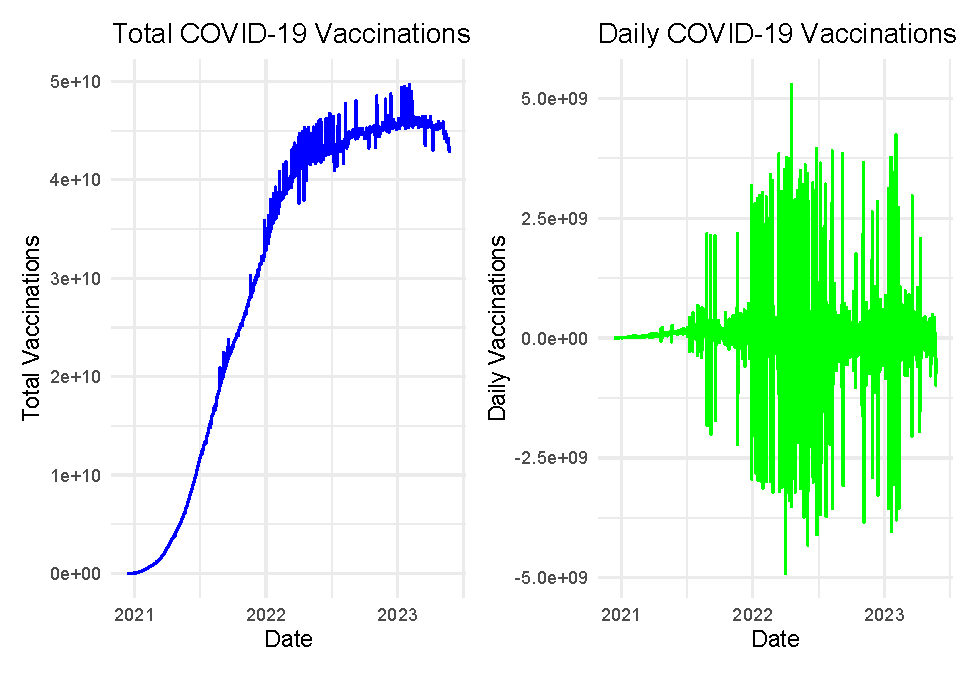
\includegraphics[height=0.6\textheight]{D:/Programowanie/R/bayesian-analysis/metProjectTemplate/metProjectTemplate_files/figure-latex/unnamed-chunk-2-1} \end{center}

By analyzing both the total and daily vaccinations, we gain a
comprehensive view of the COVID-19 vaccination progress. These
visualizations provide valuable insights into the scale and pace of
vaccinations, allowing us to evaluate the effectiveness of vaccination
campaigns and identify potential areas for improvement. \newpage

\hypertarget{top-performing-countries}{%
\section{Top Performing Countries}\label{top-performing-countries}}

Next, let's identify the top performing countries in terms of
vaccination rates and compare their progress. We will filter the latest
data for each location and sort the countries by total vaccinations.
Then, we will create a bar plot for the top 10 countries. As the dataset
contains continents and income groups, we will exclude them from the
analysis.

\vspace{1mm}
\footnotesize

\begin{flushleft}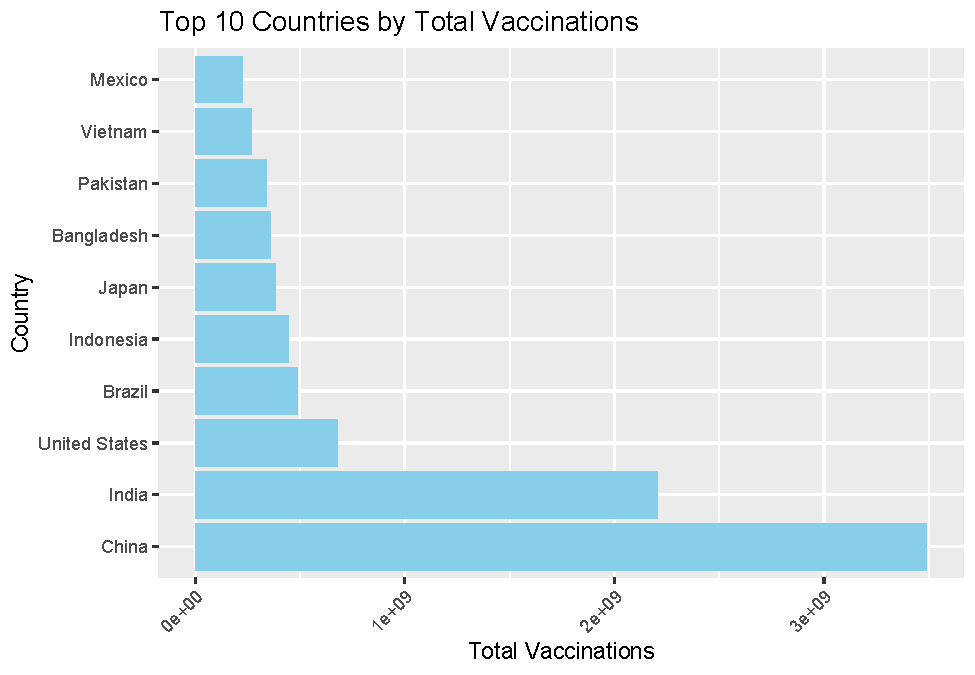
\includegraphics{D:/Programowanie/R/bayesian-analysis/metProjectTemplate/metProjectTemplate_files/figure-latex/unnamed-chunk-3-1} \end{flushleft}
\normalsize
\newpage

\hypertarget{conclusions}{%
\section*{Conclusions}\label{conclusions}}
\addcontentsline{toc}{section}{Conclusions}

\begin{itemize}
\tightlist
\item
  The global COVID-19 vaccination efforts have made significant
  progress, with numerous countries actively administering vaccinations.
\item
  Several countries emerge as leaders in terms of total vaccinations,
  demonstrating the effectiveness of their vaccination campaigns.
\item
  Daily vaccination rates show variations among different countries,
  indicating diverse approaches and strategies in vaccine distribution.
\item
  While the analysis provides valuable insights, it is essential to
  consider potential sources of errors and doubts, such as data
  accuracy, reporting inconsistencies, and variations in vaccination
  policies across countries.
\end{itemize}

By understanding the context, accessing relevant data, conducting
thorough analysis, and considering potential limitations, we can derive
meaningful insights from the COVID-19 vaccination data and contribute to
the global efforts to combat the pandemic.

\hypertarget{potential-sources-of-errors-and-doubts}{%
\section*{Potential Sources of Errors and
Doubts}\label{potential-sources-of-errors-and-doubts}}
\addcontentsline{toc}{section}{Potential Sources of Errors and Doubts}

\begin{itemize}
\tightlist
\item
  Variations in data reporting and quality across different countries
  and regions
\item
  Incomplete or missing data points that might affect the accuracy of
  the analysis
\item
  Differences in vaccination policies, distribution strategies, and
  reporting mechanisms among countries
\end{itemize}

\hypertarget{check-list}{%
\section*{Check list}\label{check-list}}
\addcontentsline{toc}{section}{Check list}

\begin{itemize}
\tightlist
\item[$\boxtimes$]
  We described the context of our problem
\item[$\boxtimes$]
  We clearly stated the questions that guided our project, and why we
  think they are important
\item[$\boxtimes$]
  We located and accessed relevant data
\item[$\boxtimes$]
  We correctly described how the data set has been obtained
\item[$\boxtimes$]
  We constructed at least two visualizations presenting the phenomenon
  that we are describing
\item[$\boxtimes$]
  We construct (with prior predictive check and posterior predictive
  check) and visualize at least one model related to the numerical
  questions we were addressing
\item[$\boxtimes$]
  We clearly explained what conclusions we are inclined to draw and why
\item[$\boxtimes$]
  We considered and clearly stated potential sources of errors and
  doubts
\end{itemize}

\end{document}
